
\section{Gemensamma erfarenheter}
Denna del tar upp diverse erfarenheter projektgruppen råkat ut för, både innan och under projektets gång.

\subsection{Erfarenheter av systemanatomi}
Systemanatomin som presenterades under \ref{beskrivning-systemanatomi} användes för att ge en enhetlig och helteckande bild över hur det färdiga systemet skulle se ut. Dock var arbetet med att ta fram själva systemanatomin något som tog relativt lång tid, om det vägs mot den nytta gruppen har haft av denna. Den blev mer ett verktyg som kunde användas för att verifiera resterande arkitekturbeskrivningar. Gruppen känner att själva processen att producera anatomin var nyttigare än den resulterande bilden, då det skapade en öppen dialog om systemets helhet.

\subsection{Tidigare erfarenheter}
Alla av projektets medlemmar hade studerat mer än två år på respektive program innan detta projekt startades. På grund av detta hade alla haft möjligheten att medverka i några större projekt och var därför ganska vana vid hur arbetet gick till. Dock var det få som hade erfarenhet med webbutveckling och spelprogrammering, något som hade stort fokus i detta projekt. Detta var dock inget större problem då de mer erfarna kunde hjälpa resten att komma igång.

\subsection{Nya erfarenheter}
Under projektets gång har alla medlemmar fått använda sig av nya verktyg och metoder som de inte haft tidigare erfarenhet av. De projektmedlemmar som tidigare saknade erfarenhet inom webbutveckling och spelprogrammering har fått chansen att sätta sig in i dessa. För att förbättra denna process hjälpte de som redan var erfarna inom ämnet till med att svara på frågor och komma med tips och idéer. Under projektets gång tillkom en del nya paket och ramverk. Ett exempel på detta är PIXI.JS, ramverket UI-applikationen använder för att rita ut spelet. Det var ingen i projektgruppen som hade jobbat med detta ramverk innan, så några i gruppen fick tillsammans sätta sig in i hur det fungerade och utbilda resterande vid behov. Detta gällde även en del av det olika npm-paketen som installerades och användes i projeket.


\subsection{Tidsbrist}
I början av projektet hade gruppen bra tidsplanering och lämnade in första iterationen i god tid för att sedan ta det lugnt. I början av iteration två satsade gruppen i huvudsak på utveckling och lämnade dokumentskrivning till senare, vilket visade sig vara en missbedömning. Detta ledde till att det blev stressigt framåt slutet av iteration två vilket kan ha påverkat dokumentkvaliteten negativt. Gruppen noterade dock detta och tog upp på kommande gruppmöten hur de skulle kunna göra det bättre inför kommande iterationer. Nästa iteration delades upp i en tydligare utvecklingsfas och dokumentfas, vilket tillät en bättre planering och fördelning av tiden.

\subsection{Tekniska erfarenheter}
Projektgruppen utvecklade applikationen i ramverket React som har något som kallas för states. Projektgruppen märkte att det snabbt kunde bli något rörigt när man introducerade flera lager av komponenter. Detta problem löser andra webbapplikationer genom extra verktyg för state-hantering, och gruppen reflekterade över dessa men beslutade emot att använda något liknande. Det visade sig dock i senare delen av projektet att hanteringen av states blev något rörig, då gruppen använt sig av fler komponenter än vad som först uppskattats. Detta ledde till att implementationen av nya komponenter som hamnade mellan redan existerande komponenter blev något jobbig. Detta berodde främst på att data som tidigare skickats från komponent \texttt{A} till \texttt{C} nu behövde skickas från \texttt{A} till \texttt{B} och sen vidare från \texttt{B} till \texttt{C}, när komponenten \texttt{B} introducerades mellan \texttt{A} och \texttt{C}. Detta ledde till att all data som tidigare skickades mellan \texttt{A} och \texttt{C} nu också behövde skickas till \texttt{B}, trots att det kunde vara data \texttt{B} inte använde sig av. En grafisk överblick kan ses i figur \ref{fig:middle_component}

\begin{figure}[H]
    \centering
    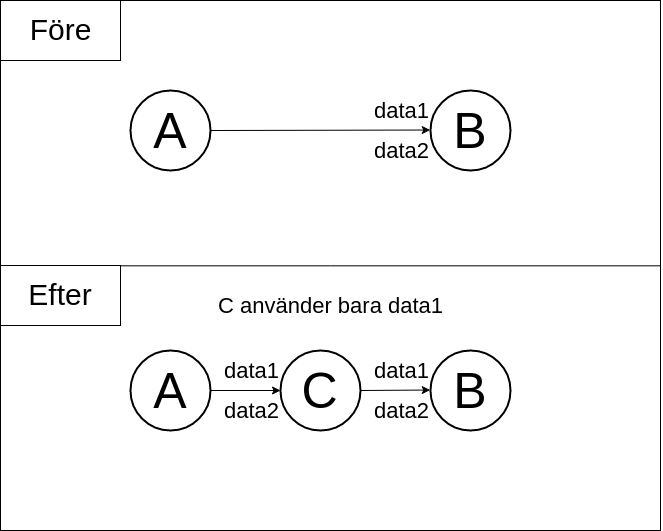
\includegraphics[scale=0.5]{middle_component}
    \caption{Överblick över hur implementation av mittenkomponent kan ge ett ineffektivt dataflöde}
    \label{fig:middle_component}
\end{figure}

\subsection{Erfarenheter med kundkontakt}
Under projekts gång har gruppen haft den stora nyttan av en nära kommunikation med kunden. Tidigt bjöds kunden in i en Slack-kanal med samtliga medlemmar, vilket ledde till en betydligt mer personlig kommunikationen än den som uppnås med mail. Gruppen har också utnyttjat kundens kontor och valt att arbeta där så mycket som möjligt. Då kunden uppmanade till att ställa frågor förtydligades diverse oklarheter snabbt vilket ledde till mer produktivt arbete. Den nära kundkontakten har också lett till en mer öppen dialog kring skapande och verifiering av produktkrav. I projektets början fördes en dialog kring krav tills kravspecifikationen ansågs vara tillräcklig. Under senare delen av projektet har kunden fått flera demonstrationer av produkten för verifiering av att den följer deras krav och vision.
